\chapter{Experimental Setup}
\label{chap:experimental_setup}

Various software environments and setups were used during the testing, extracting and evaluation of the features during this study.
We begin by describing the format of the Buckeye data set and the spectrograms, filterbanks and MFCCs extracted from it, followed by a description of the environments in which each step of the feature extraction and evaluation was performed, with specific focus on the GCP environments needed.

\section{Data set}

The Buckeye Corpus of conversational speech contains high-quality recordings from 40 speakers in Columbus OH conversing freely with an interviewer. 
The files are stored in WAV files.
Filterbank and MFCC features for spoken words within this data set were provided by Dr H. Kamper, but since spectrograms would need to be calculated as well, these features were not used. 
Instead, the word label and timestamp for these features were used to develop code to extract spectrograms, filterbanks and MFCCs and stored as Numpy files per feature type, with each individual feature as a Numpy array.

The spectrograms were calculated using a Hamming window with a frame length of 25 ms and an overlap of 15 ms.
The log value of each spectrogram was used in order to better normalise the variation in magnitudes.
This resulted in a Numpy array of size $201 \times N$, with $N \approx \frac{t}{15\times10^{-3}}$ with $t$ the time in seconds.
Filterbanks and MFCCs were calculated from these spectrograms resulting in $40 \times N$ and $39 \times N$ arrays respectively.

\section{Environments}

The bulk of the code developed for this study was written in Python 3.6, with the exception of the DTW code supplied by Dr H. Kamper\footnote{\url{https://github.com/kamperh/speech_dtw}}, which was written in Cython, and the cloud function used during the feature evaluation, which was written in Node.js v6.
Crucial libraries included Numpy, TensorFlow, Matplotlib and Scipy.

Though the language of the code was fairly consistent for this study, the different hardware requirements needed to perform the necessary tasks within a reasonable time and without any cost required some creativity, and GCP was used to accomplish many tasks that would otherwise have cost unrealistic amounts of time.

\subsection{Development}

Developing and testing of all functions were first done within a Jupyter Notebook running on a local machine.
This included the development of code to extract the spectrograms, filterbanks and MFCC features from the spoken word WAV files, configuring and alteration of the VGG16 TensorFlow model to support different input sizes as well as output the feature map of each layer, testing and altering of the code needed to perform DTW, the same-different speech task, and to calculate the AP scores.
Testing and validation of each function was also performed locally before deployment on a certain GCP service.

\subsection{Google Cloud Platform}

As described in the sections hereafter, GCP was used for various tasks in this study.
GCP is a cloud computing framework with various SaaS products.
Though these products are charged by use time, GCP offers a twelve month free trial period with \$ 300 credit, with some added limits to the use of certain products.
For the tasks needed in this study, the free trial was found to be sufficient, eliminating any costs needed for the project.
We discuss the services used in this study, namely GCE, Google Cloud Storage (GCS), Cloud Functions and Datalab.

\subsubsection{Google Compute Engine}

GCE is a service that allows users to connect remotely to a virtual machine (VM) instance.
The instance types can be tailored specifically to the user's needs by specifying the number of CPUs, the size of the memory as well as storage, the OS running on the machine and a bash script to run on start up.
API calls to create, modify and delete VM instances also exist and were used during the feature evaluation task. 

Once the instance is running, users can connect to the console via SSH to run further commands.
During the free trial of GCP, a limit of 8 vCPUs per machine is set, and a maximum of 64 CPUs in use globally.

\subsubsection{Google Cloud Storage}

GCS is a storage service for GCP products.
Files are stored in buckets, with each bucket consisting of a generic folder structure.
GCS has the added benefit of running on GCP servers, gaining read and write speeds greater than 1 GB/s from within GCP services.

For this study, all features extracted from the VGG16 network as well as the feature evaluation results were stored on GCS, resulting in $\sim$ 130 GB stored on GCS.

\subsubsection{Cloud Functions}

Cloud Functions allow for event driven server-less applications.
For the tasks in this study, Pub/Sub was used to trigger Node.js Cloud Functions.
Pub/Sub is an event streaming service that reliably transfers data to subscribed services.
Cloud Functions are a useful tool in automating GCP products, as it was used to initiate hundreds of GCE instances simultaneously during the feature evaluation task.
This process is described in detail in Section~\ref{evaluation}.

\subsubsection{Datalab}

Datalab is a service that runs a Jupyter Notebook on a specified GCE instance.
The notebook can then be accessed from a local machine, running any code within it on the GCE instance.
Though it is possible to initialise and run a Jupyter Notebook on a GCE instance normally \cite{gce}, Datalab greatly simplifies the task, as well as allow for a significant bypass of GCP limits, which is further described in Section~\ref{extraction}.

\subsection{Feature Extraction} \label{extraction}

Extracting the speech features from the VGG16 network required that the spectrograms, filterbanks and MFCCs for each spoken word be pushed through the CNN and the feature map of every filter for every layer be saved.
For the first seven convolutional layers, this meant $1\,152\times3$ different feature maps per word.
With a total of 2\,733 words, this resulted in 94\,452\,480 different features.

The problem in performing this task, is that a separate TensorFlow VGG16 graph needed to be initialised for every input feature, given that a TensorFlow graph instance can not accept different input sizes.\footnote{This was later found to be false and is detailed in Section~\ref{chap:future_work}.}
Since the features were to be stored per convolutional filter and not per spoken word, this resulted in two possible algorithms; 

A loop across the 1\,152 convolutional filters would be made each time initialising a dictionary for the current filter.
Within this loop, another loop across each of the 2\,733 words would also be made.
Within this loop, a VGG16 graph would be initialised for the given word, and only the result of a single convolutional filter would be added to the current dictionary of filters, with the key being the current word.
At the end of this loop, the current dictionary of filters would be saved as a Numpy file, and the loop would move on to the next convolutional filter.

Though this technique would keep the required memory at a given time to a minimum, the time required to initialise a TensorFlow graph and get the result of a single convolutional filter from it is roughly one second.
Having to perform this task 94\,452\,480 times would result in an execution time of over 109 days.

Instead, a loop across each of the 2\,733 words was run and the result for each of the 1\,152 filters were calculated per word and stored into separate dictionaries per filter, each saved at the end of the loop.
Though this technique required only 2\,733 TensorFlow graph initialisations resulting in less than an hour of processing time, it required the full list of 94\,452\,480 feature maps to be stored in memory for the duration of the loop.
With an average size of 10.9 kB per feature map, this algorithm would require hardware with a total memory of $\sim$ 70 GB.
Further inefficiencies within Numpy memory usage as well as having to store 2\,733 TensorFlow graphs in memory resulted in a total memory requirement of at least 210 GB.


In order to gain access to such massive memory requirements, GCP's Datalab service was required.
Though the free tier of GCE is limited to the amounts of memory and CPUs available for a single instance (30 GB and 8 vCPUs respectively), when initialised through Datalab, those limits are ignored.
Thus, a Datalab instance was initialised on a n1-highmem-64 GCE instance, resulting in 64 vCPU cores and 416 GB of memory.
The high amount of CPU cores also allowed the algorithm to be calculated simultaneously per spoken word using IPython's BackgroundJobs multithreading library.
Unfortunately though, requiring so many TensorFlow graphs to be active simultaneously and having so much memory in use, slowed down total processing time to about 24 hours.

The resulting features were then calculated on the Jupyter notebook and the resulting Numpy files copied to a GCS bucket, from which it would be available for local usage as well as to any future GCP services.
Features were stored within 3\,456 Numpy archive files, named after the specific convolutional layer and the individual filter kernel from which they were extracted, 1\,152 were extracted from the log spectrograms, 1\,152 from the filterbanks, and 1\,152 from the MFCCs. 

For the features extracted, the first two convolutional layers (\texttt{conv1\_1} and \texttt{conv1\_2}) resulted in features of the same size as the inputs that they were generated from, thus $201 \times N$ for spectrograms, $40 \times N$ for filterbanks, and $39 \times N$ for MFCCs.
\texttt{Conv2\_1} and \texttt{conv2\_2} feature maps halved each input axis, and \texttt{conv3\_1}, \texttt{conv3\_2} and \texttt{conv3\_3} quartered each input axis.
From \texttt{conv3\_1} and onward, some spoken word feature maps started becoming $X\times 1$ features, thus making the calculation of an AP score ineffective, thus layers further than \texttt{conv3\_3} were not used to extract features.

\subsection{Feature Evaluation} \label{evaluation}

In order to evaluate features using the same-different speech task, the DTW distance for each word needed to be calculated and compared to that of every other word, which, for 2\,733 words, results in 3\,733\,278 comparisons.
The time to calculate a single DTW distance on a local machine is on average 4 ms.
Even when optimised to not calculate the same DTW distance twice, this resulted in the time for a single feature type's AP score to take 4 h 8 min.
This task needed to be done for each of the 3\,456 different features, which if done sequentially would result in 1.6 years of processing time.
Experimentation also showed that multithreading this task per feature did not divide up time linearly, and would still result in a highly unrealistic time frame to complete.

In order to evaluate the features within the given time frame, each feature's AP score would truly need to be computed on a separate machine.
To accomplish this task, A Cloud Function was written that on request, instantiated a single CPU core GCE instance with preloaded instructions to download the necessary feature from GCS, run a python script to calculate and save the feature's AP score, copy the resulting file to GCS and then send a message to Pub/Sub message to instantiate another Cloud Function which would in turn destroy the GCE instance.
A script to then call a Cloud Function for each and every feature was then written and run, resulting in 3\,456 simultaneous GCE instances each computing a single feature's AP score.
Though this would have then only taken 6 h 15 min to complete, an added benefit of GCE (that it ran on Intel Skylake CPUs) resulted in the time to calculate an AP score was brought down to roughly one hour.
A visual representation of the work flow is shown in Figure~\ref{fig:workflow}.

\begin{figure}[h]
    \centering
    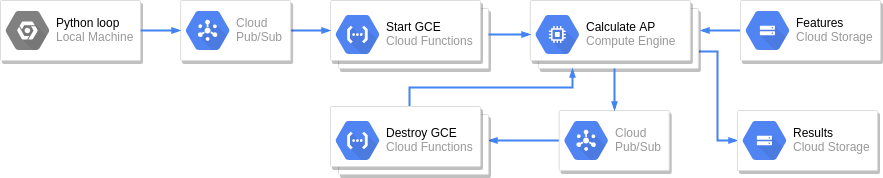
\includegraphics[width=0.9\linewidth]{content/fig/workflow.png}
    \caption{Illustrated GCP work flow to calculate AP score on individual GCE instances.}
    \label{fig:workflow}
\end{figure}

It should be noted that in order to allow for 3\,456 simultaneous GCE instances, GCP had to be taken out of the free trial period, but billing still continues from the initial \$ 300 credit.
In total, running this algorithm resulted in a cost of \$ 236.75, still staying below the allowed \$ 300 and keeping the tasks for this study without cost.